\chapter{Mathematical Preliminaries}

% ============================================================
\section{Partial Derivatives}
% ============================================================

The partial derivative of a function $F(x_1, x_2, \ldots)$ with respect to $x_1$ is defined by holding all other arguments fixed:
\begin{equation}
    \pdv{F}{x_1} = \lim_{\Delta x_1 \to 0} \frac{F(x_1 + \Delta x_1,\, x_2, \ldots) - F(x_1, x_2, \ldots)}{\Delta x_1}.
\end{equation}
In thermodynamics one frequently encounters functions of several variables where the choice of which variables to hold fixed is non-obvious, and the following identities are indispensable.

\subsection{Relations among First Partials}

Consider a function $x(y, z)$. Its total differential is
\begin{equation}
    dx = \left.\pdv{x}{y}\right|_z dy + \left.\pdv{x}{z}\right|_y dz.
\end{equation}
When $z$ is held fixed this reduces to a one-variable relationship, and the usual inverse-function theorem applies:
\begin{formula}
\begin{equation}
    \left.\pdv{x}{y}\right|_z = \left(\left.\pdv{y}{x}\right|_z\right)^{-1}.
\end{equation}
\end{formula}

A less obvious identity arises when $x$ itself is held constant. Setting $dx = 0$ gives
\begin{equation}
    0 = \left.\pdv{x}{y}\right|_z dy + \left.\pdv{x}{z}\right|_y dz,
\end{equation}
so that $dz/dy = -(\partial x/\partial y)_z / (\partial x/\partial z)_y$. Since $x$ is constant throughout, this ratio is precisely $(\partial z/\partial y)_x$, yielding the \emph{triple product rule} (also called the cyclic relation):
\begin{formula}
\begin{equation}
    \left.\pdv{x}{y}\right|_z \left.\pdv{y}{z}\right|_x \left.\pdv{z}{x}\right|_y = -1.
\end{equation}
\end{formula}
The minus sign is a recurring source of error in thermodynamics — it is worth memorising. The result is often surprising at first: three partial derivatives forming a cyclic product yield $-1$, not $+1$.

\subsection{Mixed Second Partials}

For $x(y, z)$, write $(\partial x/\partial y)_z = f_1(y,z)$ and $(\partial x/\partial z)_y = f_2(y,z)$. Provided $x$ is twice continuously differentiable, the mixed second partials commute:
\begin{equation}
    \left.\pdv{f_1}{z}\right|_y = \left.\pdv{f_2}{y}\right|_z = \frac{\partial^2 x}{\partial y\,\partial z}.
\end{equation}
This symmetry is the key to recognising exact differentials and underpins all the Maxwell relations of thermodynamics.

\subsection{Exact and Inexact Differentials}

Suppose we are given an expression $df = a(y,z)\,dy + b(y,z)\,dz$ and asked whether a function $f(y,z)$ exists whose total differential it is. A necessary and sufficient condition is that the mixed partials agree:
\begin{equation}
    \left.\pdv{a}{z}\right|_y = \left.\pdv{b}{y}\right|_z.
\end{equation}
When this holds, $df$ is called an \emph{exact differential}, and $f$ is a well-defined function of state.

If the exactness condition is satisfied, $f$ can be recovered from $df$ by the following procedure. First, integrate $a(y,z)$ with respect to $y$, keeping $z$ fixed and allowing an arbitrary function $g(z)$ to account for the undetermined $z$-dependence:
\begin{equation}
    f(y,z) = \int^y a(y', z)\,dy' + g(z).
\end{equation}
Next, differentiate with respect to $z$ and equate to $b(y,z)$:
\begin{equation}
    b(y,z) = \left.\pdv{f}{z}\right|_y = \int^y \left.\pdv{a(y',z)}{z}\right|_{y'} dy' + g'(z),
\end{equation}
which determines $g'(z)$. Integrating $g'(z)$ then gives $g(z)$ and completes the construction.

When the exactness condition fails, $df$ does not correspond to any single-valued function of state. Its integral depends on both the endpoints \emph{and} the path connecting them. Given points $P_0 = (y_0, z_0)$ and $P = (y, z)$ and a path $C$ between them, the path-dependent quantity is
\begin{equation}
    f_C(P;\,P_0) = \int_C df = \int_C \bigl(a(y',z')\,dy' + b(y',z')\,dz'\bigr).
\end{equation}
This is a line integral of the vector field $\vec{V}(y,z) = \bigl(a(y,z),\, b(y,z)\bigr)^T$. The path-dependence is most clearly seen by forming a closed loop out of two different paths $C$ and $C'$ between the same endpoints:
\begin{equation}
    f_C - f_{C'} = \oint d\vec{x}\cdot\vec{V} = \int_A d\vec{A}\cdot(\nabla\times\vec{V}),
\end{equation}
where the last step uses Stokes' theorem and
\begin{equation}
    \nabla\times\vec{V} = \left.\pdv{a}{z}\right|_y - \left.\pdv{b}{y}\right|_z.
\end{equation}
This vanishes — making the integral path-independent — if and only if $df$ is exact. Inexact differentials in thermodynamics, written with a bar ($\dbar Q$ for heat and $\dbar W$ for work), are path-dependent in precisely this sense: the total heat or work exchanged depends on \emph{how} a process is carried out, not merely on the initial and final states.

% ============================================================
\section{The Dirac Delta Function}
% ============================================================

\begin{center}
\begin{tikzpicture}[scale=0.85]
  % Axes
  \draw[->] (-2.5,0) -- (2.5,0) node[right] {$x$};
  \draw[->] (0,-0.2) -- (0,2.8) node[above] {$\delta(x-x_0)$};
  % Spike at x0
  \draw[very thick] (1.0,0) -- (1.0,2.5);
  \draw[very thick,->] (1.0,0) -- (1.0,2.6);
  % Base tick marks
  \draw (1.0,0.06) -- (1.0,-0.06) node[below] {$x_0$};
  % Axis tick
  \draw (0,0.06) -- (0,-0.06) node[below] {$0$};
\end{tikzpicture}\\[3pt]
{\small\itshape The Dirac delta $\delta(x-x_0)$: a unit-area spike at $x=x_0$.}
\end{center}

\begin{definition}[Dirac delta function]
The Dirac delta $\delta(x - a)$ is defined by the two conditions
\begin{equation}
    \delta(x - a) = 0 \quad \text{for } x \neq a,
\end{equation}
\begin{equation}
    \int_{x_0}^{x_1} \delta(x - a)\,dx =
    \begin{cases} 1 & \text{if } a \in (x_0, x_1), \\ 0 & \text{otherwise.} \end{cases}
\end{equation}
It is not a function in the classical sense but a \emph{distribution}: it is always understood inside an integral sign.
\end{definition}

The defining property of the delta function is its action on a smooth test function $f(x)$:
\begin{formula}
\begin{equation}
    \int_{x_0}^{x_1} f(x)\,\delta(x - a)\,dx = f(a), \qquad a \in (x_0, x_1).
\end{equation}
\end{formula}
Intuitively, $\delta(x-a)$ ``picks out'' the value of $f$ at $x = a$.

\subsection{Composite Arguments}

The delta function's behaviour under a change of variable is important in practice. For a linear argument $cx$, substituting $u = cx$ shows that
\begin{equation}
    \int f(x)\,\delta(cx)\,dx = \frac{1}{|c|}\,f(0),
\end{equation}
and more generally, for $\delta(cx - a)$, the zero occurs at $x = a/c$, giving
\begin{equation}
    \int f(x)\,\delta(cx - a)\,dx = \frac{1}{|c|}\,f\!\left(\frac{a}{c}\right).
\end{equation}

For a nonlinear argument $g(x)$, the delta function receives a contribution from each simple zero $x_j$ of $g$ (where $g(x_j) = 0$ and $g'(x_j) \neq 0$), with the local derivative supplying the Jacobian:
\begin{formula}
\begin{equation}
    \int f(x)\,\delta(g(x))\,dx = \sum_j \frac{f(x_j)}{|g'(x_j)|}.
\end{equation}
\end{formula}
This generalisation is used heavily when transforming probability distributions, as we shall see in Section~\ref{sec:functions-rv}.

\subsection{The Heaviside Step Function}

\begin{center}
\begin{tikzpicture}[scale=0.85]
  % --- Left panel: step function theta(x) ---
  \begin{scope}[xshift=-3.0cm]
    \draw[->] (-1.8,0) -- (1.8,0) node[right] {$x$};
    \draw[->] (0,-0.3) -- (0,1.6) node[above] {$\theta(x)$};
    % Step function
    \draw[thick,blue] (-1.7,0) -- (0,0);
    \draw[thick,blue] (0,1.0) -- (1.6,1.0);
    \draw[thick,blue,dashed] (0,0) -- (0,1.0);
    % Labels
    \draw (-0.08,1.0) -- (0.08,1.0) node[right] {$1$};
    \draw (0.06,0) -- (-0.06,0) node[below left] {$0$};
    \fill[blue] (0,1.0) circle (1.5pt);
    \fill[white] (0,0) circle (1.5pt);
    \draw[blue] (0,0) circle (1.5pt);
  \end{scope}
  % --- Right panel: delta function spike ---
  \begin{scope}[xshift=2.0cm]
    \draw[->] (-1.8,0) -- (1.8,0) node[right] {$x$};
    \draw[->] (0,-0.3) -- (0,2.0) node[above] {$\delta(x)$};
    \draw[very thick,blue,->] (0,0) -- (0,1.9);
    \draw (0.06,0) -- (-0.06,0) node[below left] {$0$};
  \end{scope}
\end{tikzpicture}\\[3pt]
{\small\itshape Left: Heaviside step function $\theta(x)$. Right: its derivative $\delta(x)$.}
\end{center}

Integrating the delta function from $-\infty$ to $x$ produces the \emph{Heaviside step function} $\theta(x)$:
\begin{equation}
    \theta(x) \equiv \int_{-\infty}^{x} \delta(x')\,dx' =
    \begin{cases} 1 & x > 0, \\ 0 & x < 0. \end{cases}
\end{equation}
Equivalently, $\dv{\theta}{x} = \delta(x)$, so the delta function is the distributional derivative of the step function. The step function is useful in practice for encoding domain constraints inside integrals, as demonstrated in Section~\ref{sec:functions-rv}.

\subsection{Representations}

Because $\delta(x)$ is not an ordinary function, it is often convenient to work with a family of smooth functions that approach it in a limiting sense. The \emph{Gaussian representation} is
\begin{equation}
    \delta_\varepsilon(x) = \frac{1}{\sqrt{2\pi}\,\varepsilon}\,e^{-x^2/2\varepsilon^2}.
\end{equation}
This has unit area for any $\varepsilon > 0$; as $\varepsilon \to 0$ the peak at the origin grows without bound while the width shrinks proportionally, so the integral remains unity and $\delta_\varepsilon \to \delta$ in the distributional sense. This representation connects directly to the Gaussian probability distribution discussed below.

% ============================================================
\section{Probability}
% ============================================================

\begin{definition}[Random variable]
A random variable $X$ is a quantity whose value cannot be predicted with certainty, but which has a definite set of possible values $\{x_j\}$. Examples include the outcome of a coin flip and the face of a die (discrete), or the speed of a gas molecule (continuous). The origin of randomness may be classical — arising from imperfect information about a deterministic system — or quantum mechanical.
\end{definition}

For a discrete random variable taking values $\{x_j\}$ with $j = 1, 2, \ldots, M$, the probability $P_j$ is defined as the limiting relative frequency:
\begin{equation}
    P_j = \lim_{N\to\infty} \frac{n_j(N)}{N}, \qquad P_j \ge 0, \qquad \sum_j P_j = 1.
\end{equation}
For a continuous random variable it is not meaningful to speak of the probability of a single exact value; instead one defines the probability density function (PDF) $p(x)$ by
\begin{definition}[Probability density]
\begin{equation}
    dP = p(x)\,dx,
\end{equation}
where $p(x) \ge 0$ and $\int_{-\infty}^\infty p(x)\,dx = 1$. The probability that $X$ lies in $[x_1, x_2]$ is $\int_{x_1}^{x_2} p(x)\,dx$.
\end{definition}

\begin{center}
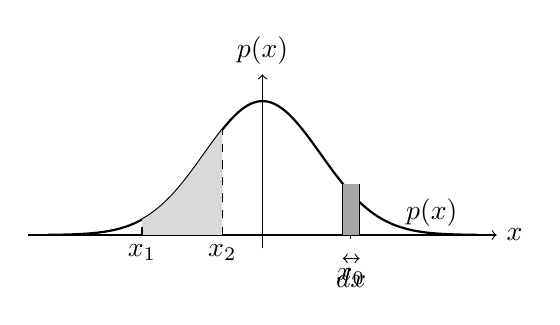
\begin{tikzpicture}[scale=0.85]
  % Axes
  \draw[->] (-3.5,0) -- (3.5,0) node[right] {$x$};
  \draw[->] (0,-0.2) -- (0,2.4) node[above] {$p(x)$};
  % Bell curve (Gaussian-like)
  \draw[thick,domain=-3.2:3.2,smooth,samples=80]
    plot (\x, {2.0*exp(-\x*\x/1.5)});
  % Shaded region from x1 to x2
  \fill[gray!30,domain=-1.8:-0.6,samples=40]
    plot (\x, {2.0*exp(-\x*\x/1.5)}) -- (-0.6,0) -- (-1.8,0) -- cycle;
  \draw[dashed] (-1.8,0) node[below] {$x_1$} -- (-1.8,{2.0*exp(-1.8*1.8/1.5)});
  \draw[dashed] (-0.6,0) node[below] {$x_2$} -- (-0.6,{2.0*exp(-0.6*0.6/1.5)});
  % Narrow strip at x0
  \fill[gray!70] (1.2,0) rectangle (1.45,{2.0*exp(-1.2*1.2/1.5)});
  \draw (1.2,0) -- (1.2,{2.0*exp(-1.2*1.2/1.5)});
  \draw (1.45,0) -- (1.45,{2.0*exp(-1.2*1.2/1.5)});
  \draw[<->] (1.2,-0.35) -- (1.45,-0.35) node[midway,below] {$dx$};
  \draw (1.32,0) -- (1.32,-0.06) node[below=0.25cm] {$x_0$};
  % p(x) label on curve
  \node[right] at (2.0,{2.0*exp(-2.0*2.0/1.5)+0.2}) {$p(x)$};
\end{tikzpicture}\\[3pt]
{\small\itshape Probability density $p(x)$: the strip $p(x_0)\,dx$ (narrow, dark) and the integral $\int_{x_1}^{x_2} p(x)\,dx$ (light shaded region).}
\end{center}

The \emph{cumulative distribution function} (CDF) is
\begin{definition}[CDF]
\begin{equation}
    \mathcal{P}(x) = \int_{-\infty}^{x} p(\xi)\,d\xi = \Pr[\text{value} < x].
\end{equation}
\end{definition}
The PDF is the derivative of the CDF: $p(x) = d\mathcal{P}/dx$.

The delta function provides a unified treatment of discrete and continuous cases. A discrete distribution $\{x_j, P_j\}$ can be described by a formal density
\begin{formula}
\begin{equation}
    p(x) = \sum_j P_j\,\delta(x - x_j),
\end{equation}
\end{formula}
which satisfies the normalization condition via the sifting property and integrates to $P_j$ over any interval containing $x_j$ alone. This formalism treats discrete, continuous, and mixed distributions within a single framework.

\subsection{Expectation Values and Moments}

\begin{definition}[Mean]
\begin{equation}
    \langle X \rangle = \int_{-\infty}^\infty x\,p(x)\,dx.
\end{equation}
\end{definition}

\begin{definition}[Variance and standard deviation]
\begin{equation}
    \mathrm{Var}(X) = \langle (X - \langle X\rangle)^2 \rangle = \langle X^2 \rangle - \langle X \rangle^2, \qquad \sigma(X) = \sqrt{\mathrm{Var}(X)}.
\end{equation}
\end{definition}
The standard deviation $\sigma$ quantifies the typical width of the distribution. Higher moments include the \emph{skewness} $\langle[(X-\langle X\rangle)/\sigma]^3\rangle$, which measures asymmetry about the mean, and the \emph{kurtosis} $\langle[(X-\langle X\rangle)/\sigma]^4\rangle$, which measures how heavy the tails are relative to a Gaussian.

\subsection{The Gaussian Distribution}

\begin{definition}[Gaussian distribution]
The Gaussian (normal) distribution is the continuous probability density
\begin{equation}
    p(x) = \frac{1}{\sqrt{2\pi\sigma^2}}\exp\!\left\{-\frac{(x-a)^2}{2\sigma^2}\right\},
\end{equation}
where $a$ is the mean and $\sigma^2$ is the variance.
\end{definition}

\begin{center}
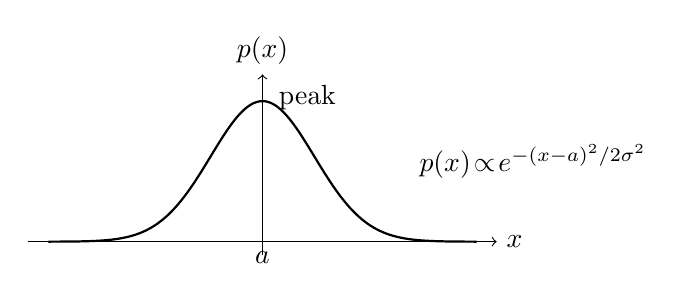
\begin{tikzpicture}[scale=0.85]
  % Axes
  \draw[->] (-3.5,0) -- (3.5,0) node[right] {$x$};
  \draw[->] (0,-0.2) -- (0,2.5) node[above] {$p(x)$};
  % Gaussian bell curve centred at a=0 (shifted for display)
  \draw[thick,domain=-3.2:3.2,smooth,samples=80]
    plot (\x, {2.1*exp(-\x*\x/1.2)});
  % Dashed vertical at peak (a)
  \draw[dashed] (0,0) -- (0,2.1);
  % Label peak
  \node[below] at (0,0) {$a$};
  \node[right] at (0.1,2.15) {peak};
  % Arrow annotation
  \node[right] at (2.2,1.2) {$p(x)\!\propto\! e^{-(x-a)^2/2\sigma^2}$};
\end{tikzpicture}\\[3pt]
{\small\itshape Gaussian distribution $p(x)\propto e^{-(x-a)^2/2\sigma^2}$ centred at $x=a$.}
\end{center}

The normalization is verified by the substitution $u = (x-a)/\sqrt{2}\,\sigma$, which brings the integral to $\pi^{-1/2}\int_{-\infty}^{\infty} e^{-u^2}\,du = 1$, using the standard result $\int_{-\infty}^{\infty} e^{-u^2}\,du = \sqrt{\pi}$. Higher moments follow by repeated differentiation under the integral sign; in particular,
\begin{equation}
    \int_{-\infty}^{\infty} u^{2n} e^{-u^2}\,du = \frac{1 \cdot 3 \cdot 5 \cdots (2n-1)}{2^n}\,\sqrt{\pi}.
\end{equation}

The cumulative distribution function is expressed in terms of the complementary error function:
\begin{equation}
    P(\bar{x}) = \frac{1}{\sqrt{2\pi\sigma^2}} \int_{-\infty}^{\bar{x}} e^{-(z-a)^2/2\sigma^2}\,dz
    = 1 - \frac{1}{2}\operatorname{erfc}\!\left(\frac{\bar{x}-a}{\sqrt{2}\,\sigma}\right),
\end{equation}
where
\begin{definition}[Complementary error function]
\begin{equation}
    \operatorname{erfc}(z) = \frac{1}{\sqrt{\pi}}\int_{z}^{\infty} e^{-u^2}\,du.
\end{equation}
\end{definition}

The parameter $\sigma$ sets the natural scale for the width. Integrating $p(x)$ over symmetric intervals about the mean gives:
\begin{align}
    \Pr(a - \sigma < x < a + \sigma) &\approx 0.68, \\
    \Pr(a - 2\sigma < x < a + 2\sigma) &\approx 0.95, \\
    \Pr(a - 5\sigma < x < a + 5\sigma) &\approx 1 - 5.7\times 10^{-7}.
\end{align}
The $5\sigma$ criterion is the standard threshold for a discovery claim in particle physics; the probability of a false positive at that level is less than one in a million.

\begin{center}
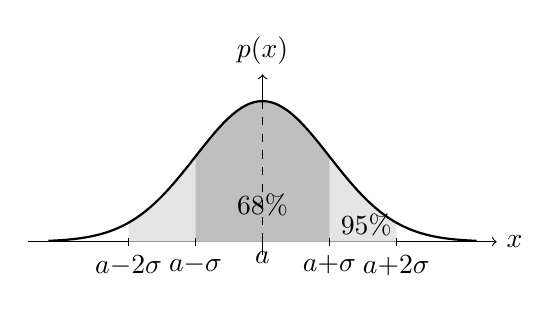
\begin{tikzpicture}[scale=0.85]
  % Axes
  \draw[->] (-3.5,0) -- (3.5,0) node[right] {$x$};
  \draw[->] (0,-0.2) -- (0,2.5) node[above] {$p(x)$};
  % 2-sigma shaded band (light gray)
  \fill[gray!20,domain=-2.0:2.0,samples=60]
    plot (\x, {2.1*exp(-\x*\x/2)}) -- (2.0,0) -- (-2.0,0) -- cycle;
  % 1-sigma shaded band (medium gray)
  \fill[gray!50,domain=-1.0:1.0,samples=40]
    plot (\x, {2.1*exp(-\x*\x/2)}) -- (1.0,0) -- (-1.0,0) -- cycle;
  % Bell curve
  \draw[thick,domain=-3.2:3.2,smooth,samples=80]
    plot (\x, {2.1*exp(-\x*\x/2)});
  % Dashed vertical at peak
  \draw[dashed] (0,0) -- (0,2.1);
  \node[below] at (0,0) {$a$};
  % sigma tick marks
  \draw (1.0,0.06) -- (1.0,-0.06) node[below] {$a{+}\sigma$};
  \draw (-1.0,0.06) -- (-1.0,-0.06) node[below] {$a{-}\sigma$};
  \draw (2.0,0.06) -- (2.0,-0.06) node[below] {$a{+}2\sigma$};
  \draw (-2.0,0.06) -- (-2.0,-0.06) node[below] {$a{-}2\sigma$};
  % Labels
  \node at (0,0.55) {68\%};
  \node at (1.55,0.25) {95\%};
\end{tikzpicture}\\[3pt]
{\small\itshape Gaussian: 68\% of probability lies within $\pm\sigma$, 95\% within $\pm 2\sigma$.}
\end{center}

\subsection{The Poisson Distribution}

\begin{definition}[Poisson process]
A Poisson process models the occurrence of discrete events in continuous time. The single assumption is that the probability of an event in a short interval $dt$ is $\lambda\,dt$, where $\lambda$ is a constant rate.
\end{definition}

Physical examples include radioactive decay and thermionic emission. Let $n$ be the number of events in total observation time $T$. To derive the probability mass function, divide $T$ into $N \gg 1$ bins each of length $T/N$, making the probability of more than one event per bin negligible. Each bin is then an independent Bernoulli trial with success probability $\lambda T/N$. Letting $z = \lambda T$ and taking $N \to \infty$, the pattern established by enumerating contributions for $n = 0, 1, 2, \ldots$ yields:

\begin{formula}[Poisson distribution]
\begin{equation}
    P_n(T) = \frac{(\lambda T)^n}{n!}\,e^{-\lambda T}.
\end{equation}
\end{formula}

Normalization follows from the Taylor series for $e^z$. The mean is computed by writing $n/n! = 1/(n-1)!$ and shifting the summation index:
\begin{equation}
    \langle n\rangle = e^{-z}\sum_{n=0}^{\infty} n\,\frac{z^n}{n!} = e^{-z}\cdot z\,e^z = z = \lambda T.
\end{equation}
For the variance, one first computes $\langle n(n-1)\rangle = z^2$ by a similar summation, obtaining $\langle n^2\rangle = z^2 + z$, and therefore:
\begin{formula}
\begin{equation}
    \mathrm{Var}(n) = \lambda T = \langle n\rangle, \qquad \sigma(n) = \sqrt{\lambda T}.
\end{equation}
\end{formula}

\begin{fact}
For the Poisson distribution, variance equals mean. The relative spread $\sigma/\langle n\rangle = 1/\sqrt{\lambda T}$ decreases with observation time; for large $\lambda T$ the distribution becomes sharply peaked.
\end{fact}

For large $\lambda T$, the Poisson distribution approaches a Gaussian. Writing $\log P_n = n\log z - \log n! - z$ and applying Stirling's approximation $\log n! \approx n\log n - n + \tfrac{1}{2}\log(2\pi n)$, one expands around the peak $n = z$ and finds the second-order term contributes $-(n-z)^2/(2z)$, giving
\begin{equation}
    P_n(z) \approx \frac{1}{\sqrt{2\pi z}}\,e^{-(n-z)^2/2z}.
\end{equation}
This is a Gaussian with mean and variance both equal to $z = \lambda T$, an instance of the Central Limit Theorem.

\subsection{The Binomial Distribution}

The binomial distribution models a random walk: a system takes $N$ steps, each independently moving right with probability $a$ or left with probability $b = 1 - a$. The random variable $n$ counts right steps.

\begin{formula}[Binomial distribution]
\begin{equation}
    P_N(n) = \binom{N}{n}(1-a)^{N-n}\,a^n.
\end{equation}
\end{formula}
The binomial coefficient $\binom{N}{n}$ counts distinct sequences with exactly $n$ right steps; each has probability $a^n(1-a)^{N-n}$.

Normalization follows from the binomial theorem: $\sum_{n=0}^{N} P_N(n) = (a+b)^N = 1$. The mean is computed using the differentiation trick $\langle n\rangle = a\,\partial_a (a+b)^N\big|_{a+b=1} = aN$. Applying the same trick to find $\langle n^2\rangle = aN + a^2N(N-1)$, one obtains:
\begin{formula}
\begin{equation}
    \langle n\rangle = Na, \qquad \mathrm{Var}(n) = Na(1-a) = Nab, \qquad \sigma(n) = \sqrt{Nab}.
\end{equation}
\end{formula}
The relative spread $\sigma/\langle n\rangle = \sqrt{(1-a)/(Na)} \to 0$ as $N\to\infty$, so relative fluctuations shrink as $1/\sqrt{N}$. For large $N$, Stirling's approximation applied to the binomial coefficients gives the Gaussian limit:
\begin{equation}
    P_N(n) \approx \frac{1}{\sqrt{2\pi Na(1-a)}}\,e^{-(n-Na)^2/2Na(1-a)},
\end{equation}
again an instance of the Central Limit Theorem: the binomial is the sum of $N$ independent Bernoulli random variables.

\begin{center}
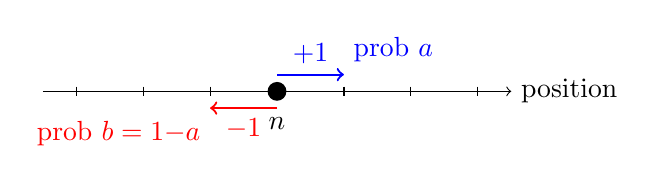
\begin{tikzpicture}[scale=0.85]
  % Number line
  \draw[->] (-3.5,0) -- (3.5,0) node[right] {position};
  % Tick marks
  \foreach \x in {-3,-2,-1,0,1,2,3} {
    \draw (\x,0.07) -- (\x,-0.07);
  }
  % Dot at current position n
  \fill[black] (0,0) circle (4pt);
  \node[below=6pt] at (0,0) {$n$};
  % Right arrow: +1 with prob a
  \draw[->,thick,blue] (0,0.25) -- (1,0.25)
    node[midway,above] {$+1$};
  \node[blue,above right] at (1,0.3) {prob $a$};
  % Left arrow: -1 with prob b
  \draw[->,thick,red] (0,-0.25) -- (-1,-0.25)
    node[midway,below] {$-1$};
  \node[red,below left] at (-1,-0.3) {prob $b=1{-}a$};
\end{tikzpicture}\\[3pt]
{\small\itshape Single random-walk step: move right with probability $a$ or left with probability $b=1-a$.}
\end{center}

\subsection{Joint Distributions, Marginals, and Statistical Independence}

When two random variables $X$ and $Y$ are present simultaneously, the appropriate object is their joint probability density:
\begin{definition}[Joint probability density]
For continuous random variables $X$ and $Y$, the joint PDF $p(x,y)$ is defined by
\begin{equation}
    p(x,y)\,dx\,dy \equiv \Pr(x \le X \le x+dx \text{ and } y \le Y \le y+dy).
\end{equation}
\end{definition}
The expected value of any function $f(x,y)$ is $\langle f\rangle = \iint dx\,dy\, f(x,y)\,p(x,y)$. The \emph{marginal distribution} for $x$ alone is obtained by integrating over all values of $y$:
\begin{equation}
    p(x) = \int_{-\infty}^{\infty} p(x,y)\,dy,
\end{equation}
and analogously for $p(y)$. The marginal $p(x)$ is the density at $x$, integrated over and therefore ignorant of all possible values of $y$.

If the joint distribution factorises as $p(x,y) = p(x)\,p(y)$, then knowledge of $y$ gives no information about $x$: the two variables are \emph{statistically independent}. In this case all joint moments factorise: $\langle f(x)\,g(y)\rangle = \langle f(x)\rangle\langle g(y)\rangle$.

\subsection{Conditional Probability and Bayes' Theorem}

Given a specific value $y$, the probability distribution for $x$ is the \emph{conditional probability} $p(x|y)$, derived from the factorisation of the joint probability element:
\begin{equation}
    p(x,y)\,dx\,dy = p(y)\,dy \cdot p(x|y)\,dx,
\end{equation}
giving
\begin{equation}
    p(x|y) = \frac{p(x,y)}{p(y)}.
\end{equation}
Since the joint distribution is symmetric, $p(x,y) = p(x|y)\,p(y) = p(y|x)\,p(x)$, one obtains immediately:

\begin{theorem}[Bayes' Theorem]
\begin{equation}
    p(y|x) = \frac{p(x|y)\,p(y)}{p(x)}.
\end{equation}
\end{theorem}
This allows one to update a prior belief $p(y)$ about $y$ given new evidence $x$, using the likelihood $p(x|y)$.

\begin{example}[Medical Testing]
A disease affects 1 in every million people, so $\Pr(D) = 10^{-6}$. A diagnostic test has sensitivity $\Pr(+|D) = 99\%$ and a false-positive rate of $1\%$, so $\Pr(+|\bar{D}) = 0.01$. If a randomly chosen person tests positive, what is $\Pr(D|+)$?

By Bayes' theorem, $\Pr(D|+) = \Pr(+|D)\,\Pr(D)/\Pr(+)$. The total probability of testing positive is
\begin{equation}
    \Pr(+) = \Pr(+|D)\Pr(D) + \Pr(+|\bar{D})\Pr(\bar{D}) \approx 0.99\times 10^{-6} + 0.01\times(1 - 10^{-6}) \approx 0.01,
\end{equation}
therefore
\begin{equation}
    \Pr(D|+) \approx \frac{0.99\times 10^{-6}}{0.01} \approx 10^{-4}.
\end{equation}
Despite a 99\% accurate test, a positive result corresponds to only about a $0.01\%$ chance of actually having the disease. The result is counterintuitive precisely because the disease is so rare: almost all positive tests come from false positives among the vast healthy population. This illustrates why base rates are essential in medical statistics.
\end{example}

% ============================================================
\section{Functions of Random Variables}
\label{sec:functions-rv}
% ============================================================

A central problem in probability is: given a random variable $X$ with density $p(x)$ and a function $Y = f(X)$, what is the density $p(y)$ of $Y$? A naive approach — simply applying the chain rule $p(y) = p(x)\,|dx/dy|$ — fails for two reasons. First, it can yield negative values, which are impossible for a density. Second, if $f$ is not monotone, multiple values of $x$ may map to the same $y$, and each pre-image must be counted.

\subsection{The Delta-Function Method}

The systematic approach starts from the identity
\begin{equation}
    p(x) = \int_{-\infty}^{\infty} p(k)\,\delta(x-k)\,dk,
\end{equation}
which recovers $p(x)$ by the sifting property. Applying the same idea to $Y = f(X)$, one integrates over all $x$ and uses the delta function to enforce $y = f(x)$:
\begin{equation}
    p(y) = \int_{-\infty}^{\infty} p(x)\,\delta\!\bigl(y - f(x)\bigr)\,dx.
\end{equation}
Using the identity $\delta(g(x)) = \sum_{x_i:\,g(x_i)=0} |g'(x_i)|^{-1}\,\delta(x-x_i)$ from Section~2, one obtains:

\begin{formula}[Density of a function of a random variable]
\begin{equation}
    p(y) = \sum_{x_i:\,f(x_i)=y} \frac{p(x_i)}{|f'(x_i)|}.
\end{equation}
\end{formula}
The sum over all pre-images $x_i$ automatically accounts for multi-valuedness; each contributes with the local stretching $|f'|$ as a Jacobian.

\subsection{Worked Example: Kinetic Energy from the Maxwell Speed Distribution}

\begin{example}[Kinetic energy from the Maxwell speed distribution]
Consider a one-dimensional gas whose molecules have velocity $v$ drawn from the Maxwell distribution $p(v) = A\,e^{-Mv^2/2k_BT}$. We want the density $p(E)$ for the kinetic energy $E = \tfrac{1}{2}mv^2$.

The map $f(v) = \tfrac{1}{2}mv^2$ is two-to-one: both $v = +\sqrt{2E/m}$ and $v = -\sqrt{2E/m}$ give the same energy $E$. Since $f'(v) = mv$, the delta-function formula gives
\begin{align}
    p(E) &= \int_{-\infty}^{\infty} dv\; p(v)\,\delta\!\bigl(E - \tfrac{1}{2}mv^2\bigr) \notag \\
         &= \sum_{v_i = \pm\sqrt{2E/m}} \frac{p(v_i)}{m|v_i|}
          = \frac{2A\,e^{-E/k_BT}}{m\sqrt{2E/m}}
          = \frac{A}{\sqrt{2mE}}\cdot 2\,e^{-E/k_BT}.
\end{align}
Both roots contribute equally in magnitude, supplying the factor of $2$ that the naive chain-rule approach misses.
\end{example}

\subsection{Worked Example: Sum of Two Uniform Variables}

\begin{example}[Sum of two uniform random variables]
For $X, Y \sim \mathrm{Uniform}[0,1]$ independently, $p(x,y) = 1$ on the unit square and zero elsewhere, and we want $p(z)$ for $Z = X + Y$. Writing the step functions explicitly to enforce the unit square,
\begin{equation}
    p(z) = \int_0^1 dx\int_{-\infty}^{\infty} dy\;\theta(y)\,\theta(1-y)\,\delta(z-x-y).
\end{equation}
Integrating over $y$ sets $y = z - x$, and the step functions restrict the $x$-integration to $x \in [\max(0, z-1),\, \min(1, z)]$. The integral over $x$ is simply the length of this interval:
\begin{align}
    0 < z < 1: &\quad p(z) = \int_0^z dx = z, \\
    1 < z < 2: &\quad p(z) = \int_{z-1}^1 dx = 2-z.
\end{align}
The result is the \emph{triangular distribution} on $[0,2]$, peaking at $z = 1$.

\begin{center}
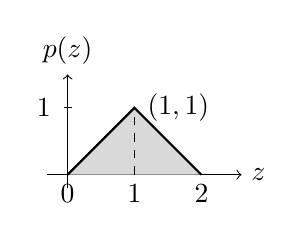
\begin{tikzpicture}[scale=0.85]
  % Axes
  \draw[->] (-0.3,0) -- (2.6,0) node[right] {$z$};
  \draw[->] (0,-0.2) -- (0,1.5) node[above] {$p(z)$};
  % Filled triangle
  \fill[gray!30] (0,0) -- (1,1) -- (2,0) -- cycle;
  % Triangle outline
  \draw[thick] (0,0) -- (1,1) -- (2,0);
  % Axis labels
  \node[below] at (0,0) {$0$};
  \node[below] at (1,0) {$1$};
  \node[below] at (2,0) {$2$};
  % Peak label
  \draw[dashed] (1,0) -- (1,1);
  \node[right] at (1.05,1.0) {$(1,1)$};
  % y-axis tick
  \draw (-0.06,1.0) -- (0.06,1.0) node[left=4pt] {$1$};
\end{tikzpicture}\\[3pt]
{\small\itshape Triangular PDF of $z=x_1+x_2$ where $x_1,x_2\sim\mathrm{Uniform}[0,1]$.}
\end{center}
\end{example}

% ============================================================
\section{Sums of Random Variables and the Central Limit Theorem}
% ============================================================

\subsection{Mean and Variance of Sums}

Let $S_n = \sum_{j=1}^{n} x_j$ be a sum of $n$ statistically independent random variables with joint density $p(x_1, \ldots, x_n) = \prod_j p_j(x_j)$. The density of $S_n$ is
\begin{equation}
    p(S_n) = \int \prod_{j=1}^{n} dx_j\, p_j(x_j)\; \delta\!\left(S_n - \sum_{j=1}^{n} x_j\right). \label{eq:sum_dist}
\end{equation}
The delta function enforces the constraint that the $x_j$ sum to $S_n$.

The mean follows immediately from the sifting property and the independence of the variables: $\langle S_n\rangle = \sum_{k=1}^{n}\langle x_k\rangle$. For the variance, one expands $\langle S_n^2\rangle$ and uses statistical independence to factorise cross terms $\langle x_k x_\ell\rangle = \langle x_k\rangle\langle x_\ell\rangle$ for $k \neq \ell$. These cross terms then cancel exactly against $\langle S_n\rangle^2$, leaving:

\begin{theorem}[Additivity of Variance]
If $x_1, \ldots, x_n$ are statistically independent, then
\begin{equation}
    \mathrm{Var}\!\left(\sum_{k=1}^{n} x_k\right) = \sum_{k=1}^{n} \mathrm{Var}[x_k].
\end{equation}
\end{theorem}
When all variables are drawn from the same distribution $p(x)$, the sample mean $\bar{x} = S_n/n$ satisfies $\langle\bar{x}\rangle = \langle x\rangle$ and $\sigma(\bar{x}) = \sigma(x)/\sqrt{n}$. Repeating a measurement $n$ times and averaging reduces the standard deviation by a factor of $\sqrt{n}$: this is why precision improves with repetition.

\begin{center}
\begin{tikzpicture}[scale=0.85]
  % --- Left panel: broad distribution p(x) ---
  \begin{scope}[xshift=-3.2cm]
    \draw[->] (-2.4,0) -- (2.4,0) node[right] {$x$};
    \draw[->] (0,-0.2) -- (0,2.2) node[above] {$p(x)$};
    % Broad Gaussian (sigma ~ 1.0)
    \draw[thick,domain=-2.2:2.2,smooth,samples=60]
      plot (\x, {1.6*exp(-\x*\x/2.0)});
    \draw[dashed] (0,0) -- (0,1.6);
    \node[below] at (0,0) {$\langle x\rangle$};
    % sigma arrow
    \draw[<->] (0,-0.5) -- (1.0,-0.5) node[midway,below] {$\sigma$};
  \end{scope}
  % --- Right panel: narrow distribution p(xbar) ---
  \begin{scope}[xshift=2.8cm]
    \draw[->] (-2.4,0) -- (2.4,0) node[right] {$\bar{x}$};
    \draw[->] (0,-0.2) -- (0,2.2) node[above] {$p(\bar{x})$};
    % Narrow Gaussian (sigma/sqrt(n) ~ 0.3)
    \draw[thick,domain=-2.2:2.2,smooth,samples=60]
      plot (\x, {2.0*exp(-\x*\x/0.18)});
    \draw[dashed] (0,0) -- (0,2.0);
    \node[below] at (0,0) {$\langle x\rangle$};
    % sigma/sqrt(n) arrow
    \draw[<->] (0,-0.5) -- (0.3,-0.5) node[midway,below] {$\tfrac{\sigma}{\sqrt{n}}$};
  \end{scope}
\end{tikzpicture}\\[3pt]
{\small\itshape CLT: the distribution of the sample mean $\bar{x}$ has standard deviation $\sigma/\sqrt{n}\ll\sigma$.}
\end{center}

\subsection{Convolutions}

The density in equation~\eqref{eq:sum_dist} is an $n$-fold convolution. For $n = 2$, the density of $S_2 = x + y$ is
\begin{equation}
    p(S_2) = \int dx\; p_1(x)\, p_2(S_2 - x),
\end{equation}
which is precisely the convolution $p_1 \circledast p_2$.

\begin{definition}[Convolution]
\begin{equation}
    (f \circledast g)(z) = \int dx\; f(x)\, g(z - x).
\end{equation}
\end{definition}

\begin{fact}
The PDF of the sum of independent random variables is the convolution of their individual PDFs.
\end{fact}

Three important families are closed under convolution. \textbf{Gaussian variables}: if $X$ and $Y$ are independently Gaussian, then $X + Y$ is Gaussian with $\langle X+Y\rangle = \langle X\rangle + \langle Y\rangle$ and $\mathrm{Var}(X+Y) = \mathrm{Var}(X) + \mathrm{Var}(Y)$. \textbf{Poissonian variables}: if $X$ and $Y$ are independently Poissonian, then $X + Y$ is Poissonian. \textbf{Lorentzian (Cauchy) variables}: the Lorentzian distribution
\begin{equation}
    p(x) = \frac{1}{\pi}\,\frac{\Gamma}{(x-a)^2 + \Gamma^2}
\end{equation}
has mean $a$ but \emph{infinite} variance (heavy tails), so the sum of Lorentzians is again Lorentzian. Because the variance is infinite, the standard deviation of the sum remains infinite regardless of how many terms are added — the Lorentzian is therefore excluded from the Central Limit Theorem.

\subsection{The Central Limit Theorem}

\begin{theorem}[Central Limit Theorem]
Let $S_n = x_1 + \cdots + x_n$ be a sum of statistically independent, identically distributed random variables each with mean $\langle x\rangle$ and finite variance $\sigma^2(x)$. As $n \to \infty$, the distribution $p(S_n)$ converges to a Gaussian:
\begin{equation}
    p(S_n) \xrightarrow{n\to\infty} \frac{1}{\sqrt{2\pi n\,\mathrm{Var}(x)}}\;\exp\!\left(-\frac{(S_n - n\langle x\rangle)^2}{2n\,\mathrm{Var}(x)}\right).
\end{equation}
The requirement of \emph{finite variance} is essential: Lorentzian distributions violate it and do not obey the CLT.
\end{theorem}

The width-to-mean ratio scales as $\sigma_{S_n}/\langle S_n\rangle \sim 1/\sqrt{n}$, so relative fluctuations vanish as $n\to\infty$ for any distribution with finite variance.

\begin{example}[Total energy of an ideal gas]
For a single atom in a one-dimensional ideal gas, the kinetic energy $E = p^2/(2m)$ has mean $\langle E\rangle = \tfrac{1}{2}k_B T$ and $\mathrm{Var}(E) = \tfrac{1}{4}(k_B T)^2$. The total energy of $N$ atoms is $E_{\text{tot}} = \sum_{i=1}^{N} E_i$, giving $\langle E_{\text{tot}}\rangle = \tfrac{1}{2}Nk_B T$ and $\mathrm{Var}(E_{\text{tot}}) = \tfrac{1}{4}N(k_B T)^2$. By the CLT, $p(E_{\text{tot}})$ becomes a sharply peaked Gaussian with relative width

\begin{center}
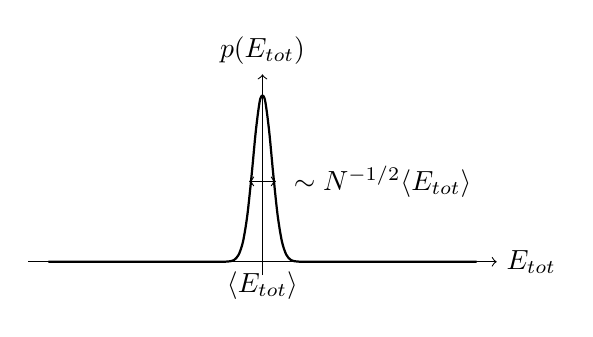
\begin{tikzpicture}[scale=0.85]
  % Axes
  \draw[->] (-3.5,0) -- (3.5,0) node[right] {$E_{\text{tot}}$};
  \draw[->] (0,-0.2) -- (0,2.8) node[above] {$p(E_{\text{tot}})$};
  % Very narrow Gaussian (width ~ 0.15)
  \draw[thick,domain=-3.2:3.2,smooth,samples=100]
    plot (\x, {2.5*exp(-\x*\x/0.04)});
  % Dashed vertical at mean
  \draw[dashed] (0,0) -- (0,2.5);
  \node[below] at (0,0) {$\langle E_{\text{tot}}\rangle$};
  % Width annotation
  \draw[<->] (-0.2,1.2) -- (0.2,1.2)
    node[right=3pt] {$\sim N^{-1/2}\langle E_{\text{tot}}\rangle$};
\end{tikzpicture}\\[3pt]
{\small\itshape The total energy of $N$ particles has extremely sharp distribution: $\sigma(E)/\langle E\rangle\sim N^{-1/2}$.}
\end{center}

\begin{equation}
    \frac{\sigma(E_{\text{tot}})}{\langle E_{\text{tot}}\rangle} = \frac{1}{\sqrt{N}} \approx 10^{-12} \quad \text{for } N \sim 10^{24}.
\end{equation}
This is an astronomically narrow peak. It is why thermodynamics deals in certainties rather than distributions: for $\sim 10^{24}$ particles, the total energy is essentially deterministic and relative fluctuations are utterly negligible. We will see this ``concentration of measure'' quantified rigorously when we derive thermodynamic entropy from counting microstates.
\end{example}

% ============================================================
\section{The Gamma Function}
% ============================================================

\begin{definition}[Gamma function]
\begin{equation}
    \Gamma(n) = \int_0^\infty x^{n-1} e^{-x}\,dx.
\end{equation}
\end{definition}
The function is well-defined for $n > 0$ and extends by analytic continuation to the entire complex plane except non-positive integers.

\subsection{Recurrence Relation and Connection to Factorials}

The base case $\Gamma(1) = \int_0^\infty e^{-x}\,dx = 1 = 0!$ is immediate. For the inductive step, integrate by parts with $u = x^{n+1}$ and $dv = e^{-x}\,dx$:
\begin{align}
    \int_0^\infty x^{n+1}e^{-x}\,dx &= \left[-x^{n+1}e^{-x}\right]_0^\infty + (n+1)\int_0^\infty x^n e^{-x}\,dx
    = (n+1)\,\Gamma(n+1),
\end{align}
where the boundary term vanishes because the exponential decays faster than any polynomial. By induction this establishes the recurrence $\Gamma(n+1) = n\,\Gamma(n)$ and the fundamental identity:
\begin{formula}
\begin{equation}
    \Gamma(n+1) = n!, \qquad n = 0, 1, 2, \ldots
\end{equation}
\end{formula}
A useful corollary, obtained by repeated differentiation under the integral sign of $\int_0^\infty e^{-tx}\,dx = 1/t$, is
\begin{formula}
\begin{equation}
    \int_0^\infty x^n e^{-tx}\,dx = \frac{n!}{t^{n+1}}, \qquad t > 0.
\end{equation}
\end{formula}

\subsection{The Special Value $\Gamma(1/2) = \sqrt{\pi}$}

Substituting $u = \sqrt{x}$ (so $x = u^2$, $dx = 2u\,du$) gives
\begin{equation}
    \Gamma\!\left(\tfrac{1}{2}\right) = \int_0^\infty x^{-1/2}e^{-x}\,dx = 2\int_0^\infty e^{-u^2}\,du \equiv 2I.
\end{equation}
To evaluate $I$, introduce the auxiliary function $f(t) = \int_0^\infty e^{-t^2(1+x^2)}/(1+x^2)\,dx$ and differentiate under the integral sign with respect to $t$:
\begin{equation}
    f'(t) = -2e^{-t^2}\int_0^\infty e^{-t^2 x^2}\,dx = -2e^{-t^2}\,I.
\end{equation}
Integrating over $t$ from $0$ to $\infty$ yields $f(\infty) - f(0) = -2I^2$. Since $f(\infty) = 0$ and $f(0) = \int_0^\infty dx/(1+x^2) = \pi/4$, one finds $I^2 = \pi/4$ and therefore:
\begin{formula}
\begin{equation}
    \Gamma\!\left(\tfrac{1}{2}\right) = \sqrt{\pi}.
\end{equation}
\end{formula}
Using the recurrence: $\Gamma(\tfrac{3}{2}) = \tfrac{1}{2}\sqrt{\pi}$, $\Gamma(-\tfrac{1}{2}) = -2\sqrt{\pi}$, and so on. These values appear frequently when normalising distributions involving half-integer powers.

\subsection{Stirling's Approximation}

For large $n$, the factorial $\Gamma(n+1) = n!$ is well approximated by expanding the integrand of $\Gamma$ around its saddle point at $x = n$. The dominant contribution gives:
\begin{formula}[Stirling's approximation]
\begin{equation}
    \log n! \approx n\log n - n + \tfrac{1}{2}\log(2\pi n).
\end{equation}
\end{formula}
In statistical mechanics one typically works with very large $n$ (of order $10^{23}$), where the correction $\tfrac{1}{2}\log(2\pi n)$ is negligible compared to the leading terms and the simpler form $\log n! \approx n\log n - n$ suffices. Stirling's approximation is essential for evaluating the entropy of large systems, for deriving the Gaussian limits of the Poisson and binomial distributions (as in the earlier sections), and for the derivation of Shannon's entropy formula.

% ============================================================
\section{Information Entropy}
% ============================================================

\subsection{Measuring Randomness}

Consider an \emph{ensemble}: a set of symbols $\{S_i\}$ together with their probabilities $\{p_i\}$. A natural measure of randomness is the minimum number of bits required to specify the value of a symbol drawn from the ensemble, on average. Two extremes clarify what is wanted. If $p_j = 1$ for one outcome and zero for all others, the outcome is certain and no bits are needed. If all $p_j$ are equal, many outcomes are plausible and more information is required. For four equally likely symbols one naively needs 2 bits per symbol, but variable-length codes that assign shorter codewords to more probable symbols can achieve a lower average when the distribution is non-uniform. Shannon's theorem identifies the fundamental limit.

\begin{theorem}[Shannon's Theorem]
The minimum average number of bits needed to transmit a signal drawn from an ensemble $\{S_i, p_i\}$ is
\begin{equation}
    \sigma = -\sum_{j=1}^{N} p_j \log_2 p_j.
\end{equation}
The quantity $\sigma$ is called the \emph{Shannon entropy} of the ensemble.
\end{theorem}

\begin{example}[Biased coin]
For $p_A = \tfrac{3}{4}$ and $p_B = \tfrac{1}{4}$, Shannon gives $\sigma = -\tfrac{3}{4}\log_2\tfrac{3}{4} - \tfrac{1}{4}\log_2\tfrac{1}{4} \approx 0.811$ bits per symbol. Encoding \emph{pairs} of symbols with a prefix-free binary tree (assigning $AA \to 0$, $AB \to 10$, $BA \to 110$, $BB \to 111$) achieves an average of $27/16 \approx 1.688$ bits per pair, or $\approx 0.844$ bits per symbol — close to the Shannon bound.

\begin{center}
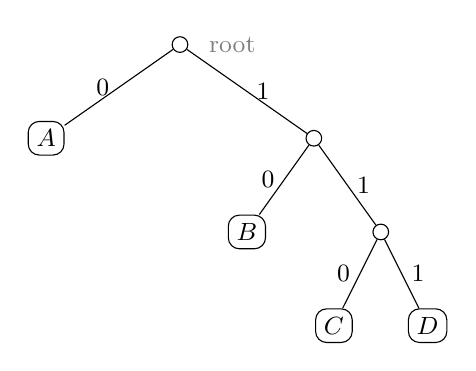
\begin{tikzpicture}[scale=0.85,
  every node/.style={font=\small},
  level 1/.style={sibling distance=4.0cm, level distance=1.4cm},
  level 2/.style={sibling distance=2.0cm, level distance=1.4cm},
  level 3/.style={sibling distance=1.4cm, level distance=1.4cm}]
  % Root
  \node[circle,draw,inner sep=2pt] (root) {}
    child {
      node[draw,rounded corners,inner sep=3pt] {$A$}
      edge from parent node[left] {$0$}
    }
    child {
      node[circle,draw,inner sep=2pt] {}
        child {
          node[draw,rounded corners,inner sep=3pt] {$B$}
          edge from parent node[left] {$0$}
        }
        child {
          node[circle,draw,inner sep=2pt] {}
            child {
              node[draw,rounded corners,inner sep=3pt] {$C$}
              edge from parent node[left] {$0$}
            }
            child {
              node[draw,rounded corners,inner sep=3pt] {$D$}
              edge from parent node[right] {$1$}
            }
          edge from parent node[right] {$1$}
        }
      edge from parent node[right] {$1$}
    };
  % Codeword labels
  \node[gray,right=4pt] at (root.east) {root};
\end{tikzpicture}\\[3pt]
{\small\itshape Prefix-free code for a biased source: $A\to0$, $B\to10$, $C\to110$, $D\to111$.}
\end{center}
\end{example}

\subsection{Derivation of the Shannon Formula}

Consider an alphabet of $N$ letters. Produce a long message of length $M \gg N$, letting letter $j$ occur $n_j$ times with $\sum_j n_j = M$. The number of distinct messages with the same letter-frequency composition is
\begin{equation}
    \Omega = \frac{M!}{n_1!\, n_2!\, \cdots\, n_N!}.
\end{equation}
To transmit one particular message one needs $B$ bits satisfying $2^B = \Omega$, so $B\log 2 = \log\Omega$. Applying Stirling's approximation,
\begin{align}
    B \log 2 &= \log M! - \sum_j \log n_j!
    \approx M\log M - \sum_j n_j \log n_j
    = -M\sum_j \frac{n_j}{M}\log\frac{n_j}{M}.
\end{align}
Identifying $p_j = n_j/M$ as the relative frequency and dividing by $M$, the minimum bits per symbol is
\begin{equation}
    \frac{B}{M} = -\sum_j p_j \log_2 p_j = \sigma,
\end{equation}
establishing Shannon's result.

\subsection{Properties of Shannon Entropy}

\begin{definition}[Shannon Entropy]
For an ensemble $\{S_i, p_i\}_{i=1}^{N}$, the Shannon entropy is
\begin{equation}
    \sigma = -\sum_{j=1}^{N} p_j \log_2 p_j,
\end{equation}
measured in bits.
\end{definition}

The minimum value $\sigma = 0$ is achieved when $p_i = 1$ for one outcome and zero for all others: no information is needed to describe a certain outcome. The maximum is achieved at the uniform distribution, $p_j = 1/N$, where $\sigma = \log_2 N$.

\begin{fact}
The uniform distribution maximises Shannon entropy subject to the normalization constraint.
\end{fact}
This follows from a Lagrange-multiplier argument: maximising $-\sum_j p_j \log p_j$ subject to $\sum_j p_j = 1$ gives $\partial/\partial p_i: \, -(\log p_i + 1) + \lambda = 0$, which is independent of $i$. By normalization $p_i = 1/N$ for all $i$, and $\sigma = \log_2 N$.

\subsection{Connection to Thermodynamic Entropy}

In information theory the probabilities $\{p_i\}$ are given. In thermodynamics, specifying a macrostate $(N, V, U)$ determines an ensemble: the macrostate is compatible with a vast number of microstates, and one does not know which microstate the system actually occupies. The thermodynamic entropy is defined as

\begin{equation}
    S = -k_B \sum_{j=1}^{\Omega} p_j \log p_j,
\end{equation}
which is the Shannon entropy rescaled: $S = k_B \ln 2 \cdot \sigma$. The differences are purely conventional — natural logarithms instead of $\log_2$, and the prefactor $k_B$ (Boltzmann's constant) introduced to match the historical unit of temperature in kelvins, so that $TS$ has dimensions of energy.

The fundamental postulate of equilibrium statistical mechanics — the ergodic hypothesis — identifies the equilibrium $\{p_j\}$ as the one that maximises $S$ subject to whatever macroscopic constraints are imposed. For an isolated system with fixed energy, volume, and particle number, all $\Omega$ compatible microstates are equally probable, and the uniform distribution gives:

\begin{formula}[Boltzmann's Entropy]
\begin{equation}
    S = k_B \log \Omega,
\end{equation}
where $\Omega$ is the multiplicity of the macrostate.
\end{formula}
This is Boltzmann's famous formula. The general relation $S = -k_B\sum_j p_j\log p_j$ is the more fundamental one; Boltzmann's formula is the special case that holds for isolated systems in equilibrium, when the maximum-entropy distribution is uniform.

Entropy is \emph{extensive}: combining two independent subsystems $A$ and $B$ with multiplicities $\Omega_A$ and $\Omega_B$ gives a combined multiplicity $\Omega_{\mathrm{tot}} = \Omega_A\cdot\Omega_B$, so $S = k_B\log(\Omega_A\Omega_B) = S_A + S_B$. Entropy is additive because the logarithm converts the multiplicative counting of independent systems into an additive quantity — a direct consequence of the statistical independence of their microstates.
